\chapter{\(k\)-Nearest Neighbor}
After having introduced all the basics of machine learning, we can start talking about the specific algorithm in order to address at the beginning of supervised classification problem. The first algorithm we present is one of the simplest one, and it is the \textbf{K-Nearest Neighbor}.

\section{Introduction}

K-Nearest Neighbor classifier is one of the introductory supervised classifiers, which every data science learner should be aware of. This algorithm was first used for a pattern classification task which was first used by Fix \& Hodges in 1951. To be similar the name was given as \(k\)-NN classifier. \(k\)-NN aims for pattern recognition tasks. The \(k\)-NN algorithm assumes that similar things exist in close proximity. In other words, similar things are near to each other.

K-Nearest Neighbor also known as \(k\)-NN is a non-parametric supervised learning algorithm that can be used for regression as well as classification problems. Generally, it is used for classification problems in machine learning. 

In \textbf{\(k\)-NN classification}, the output is a class membership. An object is classified by a plurality vote of its neighbors, with the object being assigned to the class most common among its \(k\) nearest neighbors (\(k\) is a positive integer, typically small). If \(k=1\), then the object is simply assigned to the class of that single nearest neighbor. 

In \textbf{\(k\)-NN regression} the output is the property value for the object. This value is the average of the values of \(k\) nearest neighbors.

Both for classification and regression, a useful technique can be to assign weights to the contributions of the neighbors, so that the nearer neighbors contribute more to the average than the more distant ones. For example, a common weighting scheme consists in giving each neighbor a weight of \(\frac 1 d\), where \(d\) is the distance to the neighbor.

\section{Algorithm}
\begin{wrapfigure}{l}{0.35\textwidth}
\begin{center}
    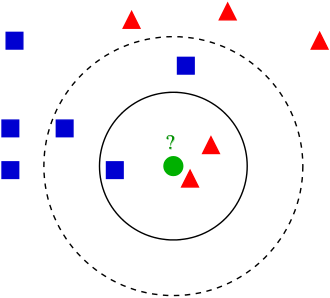
\includegraphics[width=0.35\textwidth]{029}
    \caption{}
    \label{fig:029}
\end{center}
\vspace{-40px}
\end{wrapfigure}
The training examples are vectors in a multidimensional feature space, each with a class label. The training phase of the algorithm consists only of storing the feature vectors and class labels of the training samples.

In the classification phase, \(k\) is a user-defined constant, and an unlabeled vector is classified by assigning the label which is most frequent amongh the \(k\) training samples nearest to that query point.

In Figure~\ref{fig:029} we have an example of \(k\)-NN classification. The test sample (the green dot) should be classified either to blue squares or to red triangles. if \(k=3\) (solid line circle) it is assigned to the red triangles because there are two triangles and only one square. If \(k=5\) (dashed line circle) it is assigned to the blue squares.

\subsection{Distance}
To classify an example \(d\) you have to find the \(k\) nearest neighbors of \(d\), and then choose as the label the majority label within the \(k\) nearest neighbors. But how do we measure the \emph{nearest}?

\subsubsection{Euclidean distance}
One possibility is to compute the \textbf{euclidean distance} between the test sample and  his neighbors.

In two dimensions, given two points \(A(a_1, a_2)\) and \(B(b_1, b_2)\), the euclidean distance is computed as follows:
\[D(a,b) = \sqrt{(a_1-b_1)^2 + (a_2-b_2)^2}\]

In \(n\)-dimensions, we compute the distance in an analogous manner. Given two points \(A(a_1, a_2, ..., a_n)\) and \(B(b_1, b_2, ..., b_n)\), the euclidean distance is computed as follows:
\begin{align}
D(a,b)  &= \sqrt{(a_1-b_1)^2 + (a_2-b_2)^2 + ... + (a_n-b_n)^2}\\
        &=\sqrt{\sum_{d=1}^D(a_d-b_d)^2}
\end{align}

Euclidean distance makes sense when different features are comparable, this means that each variable is measured in the same units. When features are not comparable we can standardize them by dividing by their corresponding standard deviation, this makes them all equally important. In this case we rescale the data so that the mean is 0 and the standard deviation from the mean is 1.
\begin{equation*}
    x_\text{norm} = \frac {x - \mu} {\sigma}
\end{equation*}

The min-max scaling scales the data to a fixed range between 0 and 1.
\begin{equation*}
    x_\text{norm} = \frac {x-x_\text{min}} {x_\text{max} - x_\text{min}}
\end{equation*}

The euclidean distance is the choice of the \(k\)-Nearest Neighbor algorithm.

Measuring distance (or similarity) is a domain-specific problem and there are many, many different variations. The similarity is a numberical measure of how alike two data objects are, it is higher when objects are more alike, and often falls in the range \([0,1]\). The distance is a numerical measure of how different are two data objects, it is lower when objects are more alike, and the minimum dissimilarity is often 0.

\subsubsection{Minkowski Distance}
Minkowski Distance is a generalization of the Euclidean distance.
\begin{equation}
    D(a,b) = \left[ \sum_{k=1}^p |a_k - b_k|^r \right]^{\frac 1 r}
\end{equation}
Where \(r\) is a parameter, and \(p\) is the number of dimensions. When \(r=1\) we have a city block distance (Manhatta, L1 norm); when \(r=2\) we have the euclidean distance; when \(r \to \infty\) we ahve the "supremum" distance (\(L_\infty\) norm), this is the maximum difference between any component of the vectors.

\subsubsection{Cosine Similarity}
The \textbf{cosine similarity} is defined as the cosine of the angle between the vectors, that is, the dot product of the vectors divided by the product of their lengths. It follows that the cosine similarity does not depend on the magnitudes of the vectors, but only on their angle. The cosine similarity always belongs to the interval \([-1,1]\).

\begin{equation}
S_C(A,B) := \cos(\theta) = \frac {\vec{A} \cdot \vec{B}} {||\vec{A}||\ ||\vec{B}||}
\end{equation}

Two proportional vecotrs have a cosine similarity of 1, two orthogonal vectors have a similarity of 0, and two opposite vectors have a similarity of -1.

For example, in information retrieval and text mining, each word is assigned a different coordinate and a document is represented by the vector of the numbers of occurrences of each word in the document. Cosine similarity then gives a useful measure of how similar two documents are likely to be, in terms of their subject matter, and indepently of the length of the documents.

\subsection{Pseudocode}
\begin{algorithm}
\caption{$k$-NN-classification(data, query, $k$, distance$_{fn}$)}
\label{alg:k-nn}
neighborDistance $\gets [\ ]$\;
\ForEach{$(index, example) \in data$}{
    distance $\gets$ distance$_{fn}($example.pop$()$, query$)$\;
    neigborDistance.append$(($distance$,$index$))$\;
}
sortedND $\gets$ sort$($neighborDistance$)$\;
kNNDistances $\gets$ sortedND$[k]$
\Comment*[r]{Get first $k$ neighbors}
kNNLabels $\gets [$kNNDistances.index$]$
\Comment*[r]{Get labels}
\Return{kNNDistances, Counter$($labels$)$.mostCommon$()$}
\end{algorithm}


\section{Decision boundaries}
The decision boundaries are areas, or hypersurfaces, that partitions the underlying vector space into two or more sets (one for each class); in other words is the hypersurface in the features space where the classification of a point (example) changes.

Nearest neighbor rules implicitly compute the decision boundary. It is also possible to compute the decision boundary explicitly, and to do so efficiently, so that the computational complexity is a function of the boundary complexity.

Decision boundaries are useful ways to visualize the complexity of a learned model. Intuitively, a learned model with a decision boundary that is really jagged is really complex and prone to overfitting. A learned model with a decision boundary that is really simple is potentially underfit.

In \(k\)-NN, once you have chosen \(k\), \(k\)-NN gives locally defined decision boundaries between classes, that depend on the choice of \(k\).

\section{Choosing \(k\)}

\begin{center}
    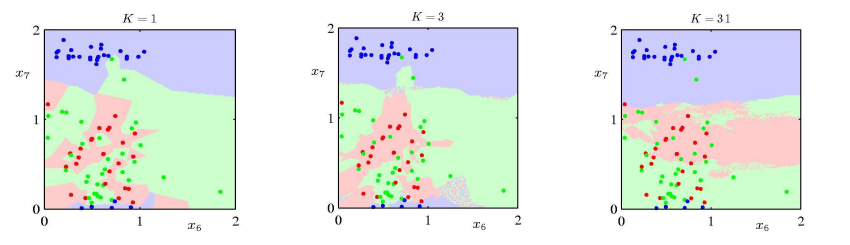
\includegraphics[width=\textwidth]{030}
    \label{fig:030}
\end{center}

The best choice of \(k\) depends upon the data; generally, larger values of \(k\) reduces effect of the noise on the classification, but make boundaries between classes less distinct. A good \(k\) can be selected by various heuristic techniques. The special case where the class is predicted to be the class of the closest training sample (i.e. when \(k=1\)) is called the nearest neighbor algorithm. Note that as we decrease the value of \(k\) to 1, our predictions become less stable, because the query point may be surrounded with noisy data that can make the prediction fail; inversely, as we increase the value of \(k\), our predictions become more stable due to majority voting, but if the number of errors begin to increase, it means that the value of \(k\) has been pushed too far.

The accuracy of the \(k\)-NN algorithm can be severely degraded by the presence of noisy or irrelevant features, or if the feature scales are not consistent with their importance. A particularly popular approach is the use of evolutionary algorithms to optimize feature scaling. Another popular approach is to scale fetures by the mutual information of the training data with the training classes. 

In binary classification problems, it is helpful to choose \(k\) to be an odd number as this avoids tied votes. One popular way of choosing the empirically optimal \(k\) in this setting is via bootstrap method.

\section{\(k\)-NN in practice}
\(k\)-NN's main disadvantage of becoming significantly slower as the volume of data increases makes it an impractical choice in environments where predictions need to be made rapidly. Moreover, there are faster algorithms that can produce more accurate classification and regression results.

However, provided you have sufficient computing resources to speedily handle the data you are using to make predictions, \(k\)-NN can still be useful in solving problems that have solutions that depend on identifying similar objects. 

At scale, this would look like recommending products on Amazon, article on Medium, movies on Netflix, or videos on YouTube. Although, we can be certain they all use more efficient means of making recommendations due to the enormous volume of data they process.

\subsection{Weighted \(k\)-Nearest Neighbor}
Weighted \(k\)-NN is a modified version of \(k\)-NN. One of the many issues that affect the performance of the \(k\)-NN algorithm is the choice of the hyperparameter \(k\). The intuition behind weighted \(k\)-NN, is to give more weight to the points which are nearby and less weight to the points which are farther away.

The \(k\)-nearest neighbor classifier can be viewed as assigning the \(k\) nearest neighbors a weight \(\frac 1 k\) and all others \(0\) weights. This can be generalized to weighted nearest neighbour classifiers. That is, where the \(i\)-th nearest neighbour is assigned a weight \(w_{ni}\) with \(\sum_{i=1}^nw_{ni}=1\). 

\subsubsection{Weighted \(k\)-NN Algorithm}
\begin{itemize}
    \item
    Let \(L=\{(x_i,y_i), i=1,2,...,n\}\) be a training set of observations \(x_i\) with given class \(y_i\), and let \(x\) be a new observation (query point) whose class label \(y\) has to be predicted.
    \item
    Compute \(d(xi,x)\) for \(i=1,2,...,n\), the distance between the query point and every other point in the training set.
    \item
    Select \(D' \subset D\), the set of \(k\) nearest training data points to the query points.
    \item
    Predict the class of the query point, using distance-weighted voting. The \(v\) represents the class labels. Use the following formula:
    \begin{equation}
        y'=argmax_v \sum_{(x_i,y_i) \in D_z}w_i \times 1(v=y_i)
    \end{equation}
\end{itemize}
Note that the function \(1\) is called \emph{indicator function}, that is defined as follows:
\begin{equation}
    1(x) = 
    \begin{cases}
        1                    &\text{if } x \text{ is true}\\
        0                    &\text{otherwise}\\
    \end{cases}
\end{equation}

\newpage
\begin{exercise}[topsep=20pt,itemsep=10pt]
    \ex Describe the \(k\)-NN algorithm.
    \ex[!] Describe the training and inference phases.
    \ex[!] Is \(k\)-NN a parametric model? Why?
    \ex How are the nearest neighbours computed? Provide the definition of the euclidean distance.
    \ex Provide the pseudocode of the \(k\)-NN classification algorithm.
    \ex What is the bottleneck at computational level of \(k\)-NN?
    \ex[!] Why does \(k\)-NN suffer from \emph{curse of dimensionality}?
    \ex What are the decision boundaries?
    \ex[!] How do we choose \(k\)?
    \ex Describe the weighted \(k\)-NN and its algorithm.
\end{exercise}